\section{Thermal Expansion}
\label{sec:thermalExpansion}

\begin{frame}{Thermal Expansion Motivation}
  \begin{itemize}
    \item Metallic fuels.
    \item PRISM designed by GE-Hitachi Nuclear Energy (GEH) \cite{GEFR793}.
    \item EBR-II designed and built by Argonne National Laboratory (ANL)
      \cite{PlentifulEnergy}.
      \begin{itemize}
        \item Full-power demonstrations from April 1986.
        \item Unprotected Loss-Of-Flow (ULOF).
        \item Unprotected Loss-Of-Heat-Sink (ULOHS).
      \end{itemize}
  \end{itemize}
\end{frame}

\begin{frame}{Simplified Thermal Expansion Model}
  \begin{itemize}
    \item FEM could be used to solve for local stresses and strains.
    \item Model is not sufficiently resolved for local temperatures.
    \item Model details.
    \begin{itemize}
      \item Calculate dimensions once at the beginning of simulation.
      \item Radial expansion modeled as steel.
      \item Axial expansion modeled as fuel.
      \item Expand all linear dimensions.
      \item Decrease local densities accordingly to preserve material.
    \end{itemize}
  \end{itemize}
\end{frame}

\begin{frame}{Material Properties}
  \begin{figure}
    \centering
    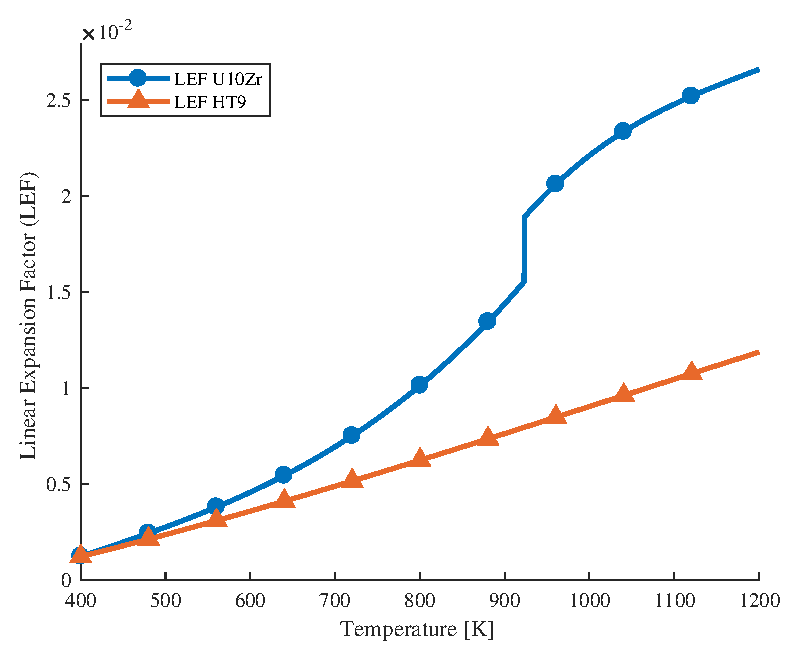
\includegraphics[width=0.7\textwidth]{lef_plot}
    \caption{Linear Expansion Factor for HT9 Steel and U10Zr Fuel.}
    \label{fig:lef_plot}
  \end{figure}
  %\begin{equation}
  %  \label{eq:lef_ht9}
  %  \left( \frac{\Delta L}{L} \right)_{\text{HT9}} = 
  %    -2.191 \times 10^{-3} + 5.678 \times 10^{-6} \, T + 
  %    8.111 \times 10^{-9} \, T^2 - 2.576 \times 10^{-12} \, T^3 ,
  %\end{equation}
  %\begin{multline}
  %  \label{eq:lef_u10zr}
  %  \left( \frac{\Delta L}{L} \right)_{\text{U10Zr}} = \\
  %    \begin{cases}
  %      -7.3 \times 10^{-3} + 3.489 \times 10^{-5} \, T 
  %        - 5.154 \times 10^{-8} \, T^2 + 4.39 \times 10^{-11} \, T^3 & 
  %        T \le 923 \units{K} \\
  %      -0.25252 + 6.669 \times 10^{-4} \, T - 5.441 \times 10^{-7} \, T^2 
  %        + 1.518 \times 10^{-10} \, T^3 & \text{otherwise}
  %    \end{cases}
  %\end{multline}
\end{frame}

\begin{frame}{Expansion Formulae}
  Given assumptions of uniform radial and axial expansion, volumes expand
  unformly.
  \begin{equation}
    \label{eq:volume_ratio}
    \frac{V^C}{V^H} = \frac{1}{(1+F_r(\texp))^2 (1+F_a(\texp))}
  \end{equation}
  Area fraction expansion ratios are more difficult and explicitly calculated in
  the code.

  To preserve the number of atoms in the reactor, the number density must be
  dilluted.
  \begin{equation}
    \label{eq:nden_thexp_update}
    N_i^H = N_i^C \frac{a_j^C}{a_j^H} 
      \frac{1}{(1+F_r(\texp))^2 (1+F_a(\texp))}
  \end{equation}
\end{frame}

\begin{frame}{Demonstration of Reactor Thermal Expansion}
  \begin{figure}
    \centering
    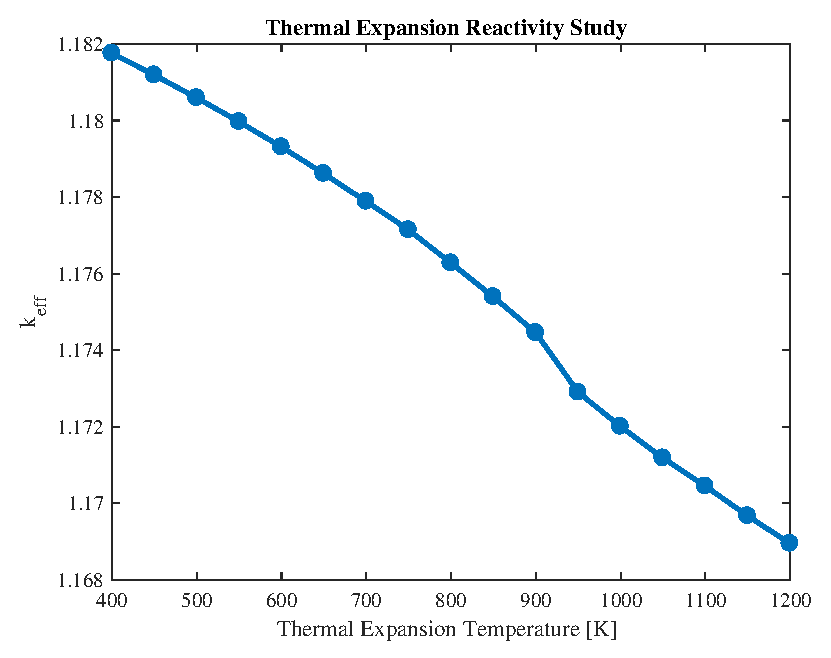
\includegraphics[width=0.7\textwidth]{thexp_study}
    \caption{Effective Neutron Multiplication Factor as a Function of 
      Thermal Expansion Temperature.}
    \label{fig:thexp_study}
  \end{figure}
\end{frame}
